% ============================================================
%  Poster : Crank-Nicolson Method for the TDSE
%  Engine : pdflatex  |  Class: tikzposter
%  Size: A0 landscape
% ============================================================
\documentclass[20pt, a0paper, landscape]{tikzposter}

% == Core packages ===========================================
\usepackage[T1]{fontenc}
\usepackage{lmodern}
\usepackage{amsmath,amssymb,bm,mathtools}
\usepackage{booktabs}
\usepackage{array}
\usepackage{graphicx}
\usetikzlibrary{arrows.meta, shapes.geometric, positioning,
                fit, calc, decorations.pathreplacing, shadows}

% ============================================================
%  COLOUR PALETTE  -  "Paper Daylight"
% ============================================================
%  Backgrounds
\definecolor{BgPage}      {HTML}{F8F7F2}   % warm paper
\definecolor{BgBlock}     {HTML}{FFFFFF}   % clean white
\definecolor{BgTitle}     {HTML}{E7EEF7}   % cool mist blue
\definecolor{BgInnerT}    {HTML}{EFE7D8}   % warm sand
\definecolor{BgInner}     {HTML}{F6F4EF}   % soft paper
%  Text
\definecolor{TxtMain}     {HTML}{1B1E23}   % near-black
\definecolor{TxtDim}      {HTML}{4B5563}   % muted graphite
%  Accents
\definecolor{Aqua}        {HTML}{0F6FA6}   % deep blue
\definecolor{Gold}        {HTML}{B88300}   % muted gold
\definecolor{Mint}        {HTML}{0F7A5B}   % deep green
\definecolor{Coral}       {HTML}{B4433E}   % brick red
\definecolor{Lavender}    {HTML}{5D5CCF}   % subdued violet
\definecolor{TitleLine1}  {HTML}{0F6FA6}   % title blue
\definecolor{TitleLine2}  {HTML}{7A4E00}   % title gold

% == tikzposter color wiring =================================
\usetheme{Default}

\definecolorstyle{PaperStyle}{}{
  \colorlet{backgroundcolor}    {BgPage}
  \colorlet{framecolor}         {Aqua}
  \colorlet{titlefgcolor}       {TxtMain}
  \colorlet{titlebgcolor}       {BgTitle}
  \colorlet{blocktitlebgcolor}  {BgTitle}
  \colorlet{blocktitlefgcolor}  {TxtMain}
  \colorlet{blockbodybgcolor}   {BgBlock}
  \colorlet{blockbodyfgcolor}   {TxtMain}
  \colorlet{innerblocktitlebgcolor}{BgInnerT}
  \colorlet{innerblocktitlefgcolor}{TxtMain}
  \colorlet{innerblockbodybgcolor} {BgInner}
  \colorlet{innerblockbodyfgcolor} {TxtMain}
  \colorlet{notefgcolor}        {TxtMain}
  \colorlet{notebgcolor}        {Gold}
  \colorlet{noteframecolor}     {Gold}
}
\usecolorstyle{PaperStyle}
\usetitlestyle{Filled}
\useblockstyle{Slide}
\useinnerblockstyle{Table}

% == Title ===================================================
\settitle{
  \vspace{3mm}
  % Left Block: Names and Entry Numbers
  \begin{minipage}[c]{0.28\linewidth}
    \begin{flushleft}
      \textcolor{TitleLine1}{\Large\textbf{Abhinav P J}} \hspace{0.5em} \textcolor{TxtMain}{\Large 2024CS10924} \\[3mm]
      \textcolor{TitleLine1}{\Large\textbf{Harsh Verma}} \hspace{0.5em} \textcolor{TxtMain}{\Large 2024CS10499} \\[3mm]
      \textcolor{TitleLine1}{\Large\textbf{Sainavaneet Mukund}} \hspace{0.5em} \textcolor{TxtMain}{\Large 2024CS10025}
    \end{flushleft}
  \end{minipage}%
  % Center Block: Main Poster Title
  \begin{minipage}[c]{0.44\linewidth}
    \centering
    {\bfseries\fontsize{54}{60}\selectfont\color{TitleLine1}
      Solving the Time-Dependent Schr\"{o}dinger Equation}\\[4mm]
    {\bfseries\fontsize{36}{42}\selectfont\color{TitleLine2}
      via the Crank--Nicolson Method:\; Stability,\; Unitarity \& Efficient Linear Algebra}\\[3mm]
    {\large\color{TxtDim}\itshape
      A complete mathematical derivation from operator formalism
      to tridiagonal linear systems and the Thomas algorithm}
  \end{minipage}%
  % Right Block: QR Code
  \begin{minipage}[c]{0.28\linewidth}
    \begin{flushright}
      
\includegraphics[width=4.5cm]{qr.png} \\[2mm]
      \textcolor{TxtMain}{\Large\textbf{GitHub}}
    \end{flushright}
  \end{minipage}
  \vspace{3mm}
}

% == Macros ==================================================
\renewcommand{\Psi}{\varPsi}
\newcommand{\dt}{\Delta t}
\newcommand{\dx}{\Delta x}
\newcommand{\calO}{\mathcal{O}}
\newcommand{\bPsi}{\bm{\Psi}}
\newcommand{\half}{\tfrac{1}{2}}

% == Reduce spacing above \innerblock ========================
\NewCommandCopy{\oldinnerblock}{\innerblock}
\renewcommand{\innerblock}[3][]{%
  \par\vspace{-12mm}% <--- Adjust this negative value (-10mm, -15mm, etc.)
  \oldinnerblock[#1]{#2}{#3}%
}
% ============================================================
\begin{document}
\maketitle[titletotopverticalspace=3mm,
           titletoblockverticalspace=6mm]




% ============================================================
\begin{columns}
% ============================================================
%  COLUMN 1  (26%)  -  Physics, Discretization & Euler Schemes
% ============================================================
\column{0.29}

% == 1. Physical Problem =====================================
\block{1.\enspace The Physical Problem}{

The \textbf{Time-Dependent Schr\"{o}dinger Equation} (TDSE) governs
quantum state evolution:
\begin{equation}
  \boxed{i\hbar\,\frac{\partial \Psi(x,t)}{\partial t}
  = \hat{H}\,\Psi(x,t)
  = \left[-\frac{\hbar^2}{2m}\frac{\partial^2}{\partial x^2}
    + V(x)\right]\Psi(x,t)}
\end{equation}

\textbf{Formal solution} - time-evolution operator:
\[
  \Psi(x,t{+}\dt) \;=\;
  \underbrace{e^{-i\hat{H}\dt/\hbar}}_{\displaystyle\hat{U}(\dt)}\,\Psi(x,t)
\]

\innerblock{\textbf{Unitarity: the Core Requirement}}{
  $\hat{H} = \hat{H}^\dagger$ (Hermitian) $\Rightarrow$
  $\hat{U}^\dagger\hat{U} = e^{+i\hat{H}\dt/\hbar}e^{-i\hat{H}\dt/\hbar} = \hat{I}$\\[4pt]
  This enforces \textbf{probability conservation}:
  \[
    \int_{-\infty}^{+\infty}|\Psi(x,t)|^2\,dx = 1\quad\forall\, t
  \]
  \textit{Any valid numerical scheme must discretely replicate this.}
}

\vspace{2mm}
The computational challenge: approximate $e^{-i\hat{H}\dt/\hbar}$
on a finite spatial grid while keeping the discrete propagator \emph{exactly} unitary.
}

% == 2. Discretization =======================================
\block{2.\enspace Space--Time Discretization}{

Introduce a uniform grid with $N+1$ spatial and $M$ temporal points:
\[
  x_j = j\,\dx,\;\;
  j=0,\ldots,N;\qquad
  t_n = n\,\dt,\;\; n=0,1,\ldots
\]

\textbf{Central finite difference} ($2^{\rm nd}$-order, $\calO(\dx^2)$):
\begin{equation}
  \left.\frac{\partial^2\Psi}{\partial x^2}\right|_{x_j}
  \approx
  \frac{\Psi_{j+1}^n - 2\Psi_j^n + \Psi_{j-1}^n}{(\dx)^2}
\end{equation}

\textit{Derived by Taylor expansion:}\;
$\Psi_{j\pm1} = \Psi_j \pm \dx\Psi' + \frac{(\dx)^2}{2}\Psi'' \pm \frac{(\dx)^3}{6}\Psi''' + \calO(\dx^4)$

\medskip
The \textbf{discrete Hamiltonian} $H_{FD}$ acts on the grid vector
$\bPsi^n = [\Psi_1^n,\ldots,\Psi_{N-1}^n]^{\mathsf T}$:
\[
  (H_{FD}\bPsi^n)_j
  = -\beta\Psi_{j-1}^n + (2\beta + V_j)\Psi_j^n - \beta\Psi_{j+1}^n,
  \quad
  \beta \equiv \frac{\hbar^2}{2m(\dx)^2}
\]

\innerblock{Boundary Conditions}{
\begin{tabular}{@{}ll}
  \textcolor{Gold}{\textbf{Dirichlet}} (infinite well): &
    $\Psi_0^n = \Psi_N^n = 0$\\[3pt]
  \textcolor{Lavender}{\textbf{Periodic}} (ring/lattice): &
    $\Psi_0^n = \Psi_{N}^n,\;\Psi_{-1}^n=\Psi_{N-1}^n$\\[3pt]
  \textcolor{Coral}{\textbf{Absorbing}} (open boundary): &
    Add $-i\Gamma(x)$ to $V(x)$ near edges
\end{tabular}
}
}

% == 3. Method Comparison ====================================
\block{3.\enspace Why Euler Schemes Fail}{
{\raggedright
\textbf{Stability test:} substitute $\Psi_j^n = g^n e^{ik j\dx}$
(Fourier mode) into each scheme and compute amplification factor~$g$.\par
}
\vspace{4mm}
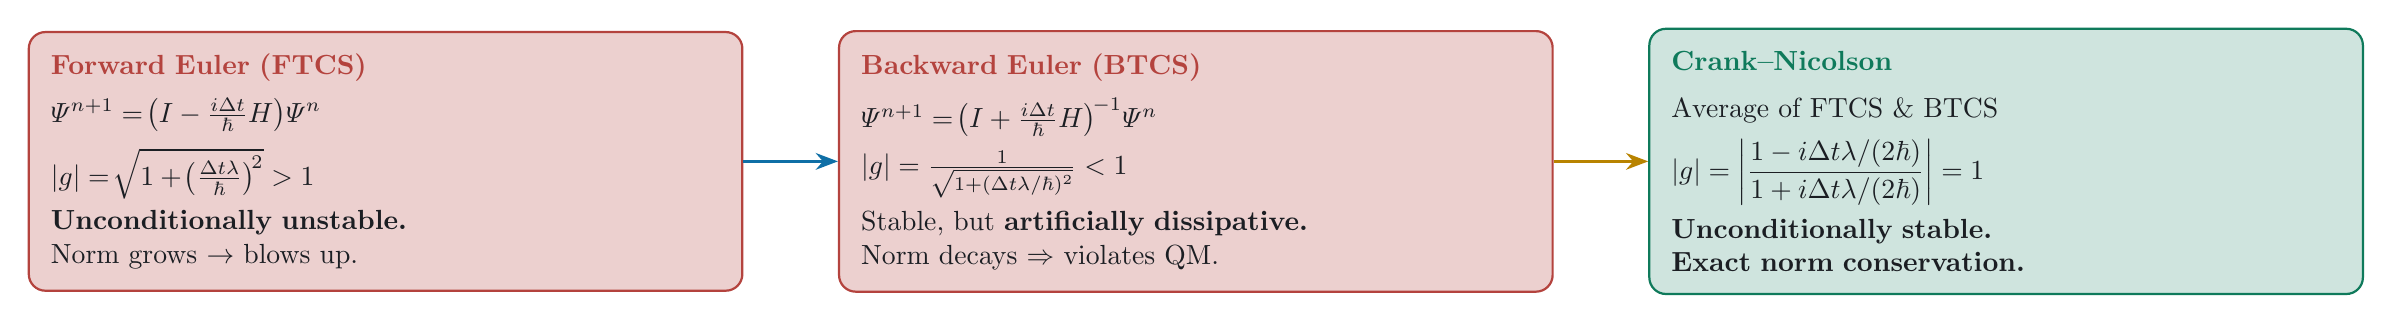
\begin{tikzpicture}[
  every node/.style={font=\normalsize},
  mbox/.style={draw, rounded corners=6pt, thick,
               minimum height=3.2cm, text width=8.5cm,
               align=left, inner sep=8pt},
  rbox/.style={mbox, draw=Coral, fill=Coral!25, text=TxtMain},
  gbox/.style={mbox, draw=Mint,  fill=Mint!20,  text=TxtMain},
  arr/.style={-{Stealth[length=8pt]}, very thick},
]
  \node[rbox] (fe) {
    \textcolor{Coral}{\textbf{Forward Euler (FTCS)}}\\[5pt]
    $\Psi^{n+1} = \!\left(I - \frac{i\dt}{\hbar}H\right)\!\Psi^n$\\[5pt]
    $|g| = \!\sqrt{1+\!\left(\frac{\dt\lambda}{\hbar}\right)^{\!2}} > 1$\\[4pt]
    \textbf{Unconditionally unstable.}\\
    Norm grows $\to$ blows up.
  };
  \node[rbox, right=12mm of fe] (be) {
    \textcolor{Coral}{\textbf{Backward Euler (BTCS)}}\\[5pt]
    $\Psi^{n+1} = \!\left(I + \frac{i\dt}{\hbar}H\right)^{\!-1}\!\Psi^n$\\[5pt]
    $|g| = \frac{1}{\sqrt{1+(\dt\lambda/\hbar)^2}} < 1$\\[4pt]
    Stable, but \textbf{artificially dissipative.}\\
    Norm decays $\Rightarrow$ violates QM.
  };
  \node[gbox, right=12mm of be] (cn) {
    \textcolor{Mint}{\textbf{Crank--Nicolson}}\\[5pt]
    Average of FTCS \& BTCS\\[5pt]
    $|g| = \left|\dfrac{1 - i\dt\lambda/(2\hbar)}
                       {1 + i\dt\lambda/(2\hbar)}\right| = 1$\\[4pt]
    \textbf{Unconditionally stable.}\\
    \textbf{Exact norm conservation.}
  };
  \draw[arr, color=Aqua]  (fe.east) -- (be.west)
    node[midway,above,font=\small,color=Aqua]{};
  \draw[arr, color=Gold]  (be.east) -- (cn.west)
    node[midway,above,font=\small,color=Gold]{};
\end{tikzpicture}

\vspace{2mm}
Here $\lambda$ denotes any eigenvalue of $H_{FD}$; since $H_{FD}$ is
real-symmetric all eigenvalues are real, so $|g|=1$ holds for
\emph{every} mode simultaneously - unconditional stability.
}

% ============================================================
%  COLUMN 2  (37%)  -  CN Derivation & Matrix Structure
% ============================================================
\column{0.34}

% == 4. Operator Approximation ===============================
\block{4.\enspace Crank-Nicolson \& the Pad\'e Approximants }{
Instead of evaluating the derivative at the current \emph{or} future
time alone, Crank-Nicolson evaluates the TDSE at the \textbf{temporal midpoint}
$t_{n+1/2}$ by averaging the Hamiltonian at both levels:
\begin{equation}
  i\hbar\,\frac{\Psi_j^{n+1}-\Psi_j^n}{\dt}
  \;=\;
  \tfrac{1}{2}\!\left(H_{FD}\Psi_j^{n+1} + H_{FD}\Psi_j^n\right)
  \label{eq:cn}
\end{equation}
\\
\\
The exact time-evolution operator is $\hat{U} = e^{-ix}$, where $x \equiv \hat{H}\dt/\hbar$. 
Direct computation of the matrix exponential $e^{-i\hat{H}\dt/\hbar}$ is impractically expensive. 
Instead, the Crank--Nicolson method employs the \textbf{Pad\'e [1,1] approximant}:
\begin{equation}
  e^{-ix} \;\;\approx\;\; R(x) \;=\; \frac{1 - ix/2}{1 + ix/2} \quad \implies \quad U_{CN} = \left(I + i\frac{\dt}{2\hbar}H\right)^{\!-1}\!\left(I - i\frac{\dt}{2\hbar}H\right)
\end{equation}

\innerblock{\textbf{Taylor Series Matching (Order of Accuracy)}}{
Let's compare their expansions for a small time step $x$:
\begin{align*}
  \textcolor{Aqua}{\text{Exact:}\quad e^{-ix}} &= 1 - ix - \frac{x^2}{2} + i\frac{x^3}{6} + \mathcal{O}(x^4) \\[4pt]
  \textcolor{Gold}{\text{Pad\'e:}\quad R(x)} &= \left(1 - i\frac{x}{2}\right)\left(1 - i\frac{x}{2} - \frac{x^2}{4} + i\frac{x^3}{8} + \dots\right) \\
  &= 1 - ix - \frac{x^2}{2} + i\frac{x^3}{4} + \mathcal{O}(x^4)
\end{align*}
The expressions \textbf{match exactly up to $\mathcal{O}(x^2)$}. The discrepancy begins at the $\mathcal{O}(x^3)$ term, meaning the local truncation error per step is $\mathcal{O}(\dt^3)$. This makes the method \textbf{globally 2nd-order accurate} in time.
}

}

% == 5. Matrix Structure =====================================
\block{5.\enspace Tridiagonal Matrix Structure of $A$ and $B$}{

Let $r_j \equiv \gamma(2\beta+V_j)$ (diagonal) and $s \equiv \gamma\beta$
(off-diagonal) with $\gamma = \dt/(2\hbar)$. The linear system \eqref{eq:linsys} reads:

\begin{equation}
\label{eq:linsys}
\underbrace{
\!\begin{pmatrix}
  1{+}ir_1 & -is      & 0        & \cdots & 0 \\
  -is      & 1{+}ir_2 & -is      & \cdots & 0 \\
  0        & -is      & 1{+}ir_3 & \cdots & 0 \\
  \vdots   &          &          & \ddots & -is \\
  0        & 0        & \cdots   & -is    & 1{+}ir_{N-1}
\end{pmatrix}
}_{A}\!
\bPsi^{n+1}
=
\underbrace{
\!\begin{pmatrix}
  1{-}ir_1 & +is      & 0        & \cdots & 0 \\
  +is      & 1{-}ir_2 & +is      & \cdots & 0 \\
  0        & +is      & 1{-}ir_3 & \cdots & 0 \\
  \vdots   &          &          & \ddots & +is \\
  0        & 0        & \cdots   & +is    & 1{-}ir_{N-1}
\end{pmatrix}
}_{B}\!
\bPsi^{n}
\end{equation}

\innerblock{\textbf{Expanding the Discrete Hamiltonian}}{
Substituting $H_{FD}\Psi_j = -\beta\Psi_{j-1} + (2\beta+V_j)\Psi_j
- \beta\Psi_{j+1}$ into both sides of \eqref{eq:linsys},
grouping by spatial index $j{-}1$, $j$, $j{+}1$:

\smallskip
\textbf{Left side} (future unknowns $\Psi^{n+1}$):
\[
  \textcolor{Aqua}{(-i\gamma\beta)}\,\Psi_{j-1}^{n+1}
  + \textcolor{Aqua}{\bigl[1 + i\gamma(2\beta+V_j)\bigr]}\,\Psi_j^{n+1}
  + \textcolor{Aqua}{(-i\gamma\beta)}\,\Psi_{j+1}^{n+1}
\]
\textbf{Right side} (present knowns $\Psi^{n}$):
\[
  \textcolor{Gold}{(+i\gamma\beta)}\,\Psi_{j-1}^{n}
  + \textcolor{Gold}{\bigl[1 - i\gamma(2\beta+V_j)\bigr]}\,\Psi_j^{n}
  + \textcolor{Gold}{(+i\gamma\beta)}\,\Psi_{j+1}^{n}
\]
}

% --- THREE SIDE-BY-SIDE IMAGES IMPLEMENTATION ---


\begin{minipage}{0.32\linewidth}
    \centering
    \includegraphics[width=\linewidth]{frame_0128.png}
    
    {\small (a) Frame 1}
\end{minipage}\hfill
\begin{minipage}{0.32\linewidth}
    \centering
    \includegraphics[width=\linewidth]{frame_0290.png}
    
    {\small (b) Frame 2}
\end{minipage}\hfill
\begin{minipage}{0.32\linewidth}
    \centering
    \includegraphics[width=\linewidth]{frame_0329.png}
    
    {\small (c) Frame 3}
\end{minipage}


}

% ============================================================
%  COLUMN 3  (37%)  -  Thomas Algorithm, Complexity, Summary
% ============================================================
\column{0.37}

% == 6. Thomas Algorithm =====================================
\block{6.\enspace Thomas Algorithm - $\calO(N)$ Tridiagonal Solver}{

Naïve LU decomposition costs $\calO(N^3)$.
The Thomas algorithm exploits the \textbf{tridiagonal structure} to achieve
$\calO(N)$ with only $\approx 8N$ floating-point operations - no fill-in.
\medskip

Let the system be $a_j\Psi_{j-1} + d_j\Psi_j + c_j\Psi_{j+1} = f_j$
with $a_j = c_j = -is$, $d_j = 1+ir_j$.

\innerblock{\textbf{Step 1 - Forward Sweep} (modify coefficients)}{
Initialise: $\tilde d_1 = d_1,\; \tilde f_1 = f_1$.\\[4pt]
For $j = 2, 3, \ldots, N{-}1$:
\[
  m_j = \frac{a_j}{\tilde d_{j-1}},
  \qquad
  \tilde d_j = d_j - m_j\, c_{j-1},
  \qquad
  \tilde f_j = f_j - m_j\, \tilde f_{j-1}
\]
Eliminates the sub-diagonal in $\calO(N)$ steps.
}

\vspace{2mm}
\innerblock{\textbf{Step 2 - Back Substitution} (recover $\bPsi^{n+1}$)}{
\[
  \Psi_{N-1}^{n+1} = \frac{\tilde f_{N-1}}{\tilde d_{N-1}},
  \qquad
  \Psi_j^{n+1} = \frac{\tilde f_j - c_j\,\Psi_{j+1}^{n+1}}{\tilde d_j},
  \quad j = N{-}2,\ldots,1
\]
}

\vspace{4mm}
\textbf{Full time-stepping algorithm:}

\begin{center}
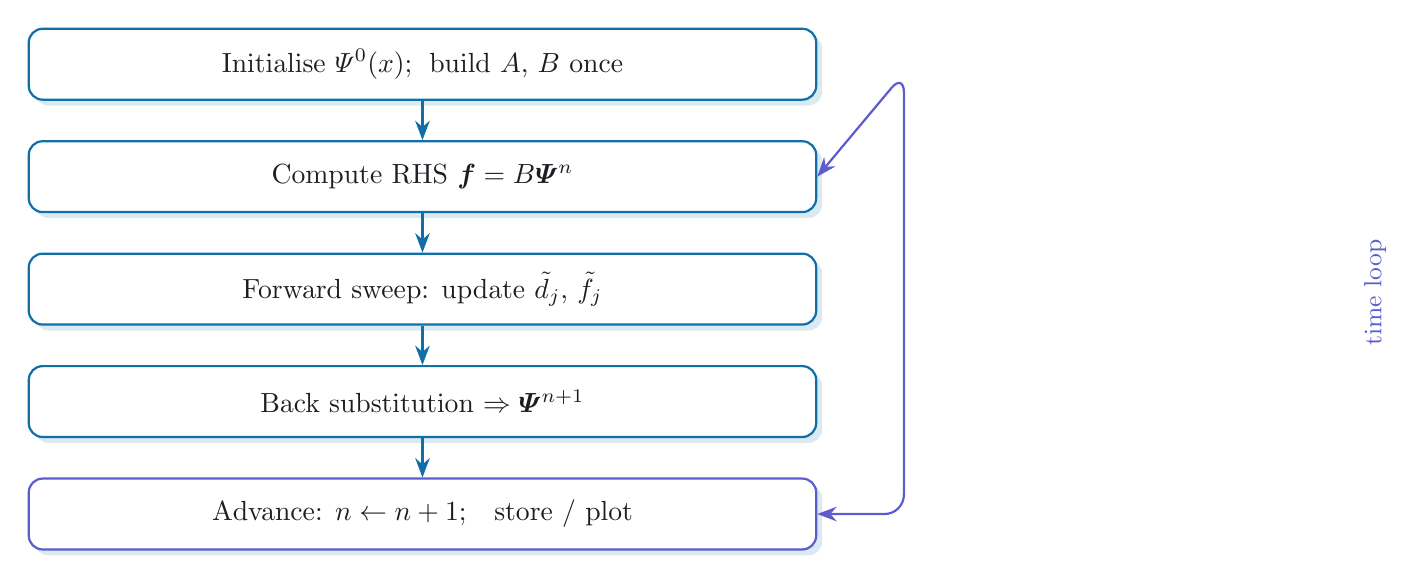
\begin{tikzpicture}[
  node distance=5mm,
  every node/.style={font=\normalsize},
  flowstep/.style={draw=Aqua, fill=BgBlock, rounded corners=5pt, thick,
               text=TxtMain, minimum width=10cm, minimum height=9mm,
               align=center, drop shadow={color=Aqua!30}},
  check/.style={flowstep, draw=Gold, fill=BgBlock},
  loop/.style={flowstep, draw=Lavender, fill=BgBlock},
  arr/.style={-{Stealth[length=7pt]}, thick, color=Aqua},
]
  \node[flowstep]  (init) {Initialise $\Psi^0(x)$;\; build $A$, $B$ once};
  \node[flowstep, below=of init]  (rhs)  {Compute RHS $\bm f = B\bPsi^n$};
  \node[flowstep, below=of rhs]   (fwd)  {Forward sweep: update $\tilde d_j$, $\tilde f_j$};
  \node[flowstep, below=of fwd]   (bak)  {Back substitution $\Rightarrow \bPsi^{n+1}$};
  \node[loop, below=of bak]   (adv)  {Advance: $n \leftarrow n+1$;\quad store / plot};

  \foreach \a/\b in {init/rhs, rhs/fwd, fwd/bak, bak/adv}
    \draw[arr] (\a) -- (\b);

  % loop-back arrow
  \draw[{Stealth[length=7pt]}-{Stealth[length=7pt]},
        thick, color=Lavender, rounded corners=7pt]
    (adv.east) -- ++(1.1,0) -- ++(0,5.6) -- (rhs.east);
  \node[color=Lavender, font=\small, rotate=90] at (12.1, -2.9)
    {time loop};
\end{tikzpicture}
\end{center}
}

% == 7. Complexity Table =====================================
\block{7.\enspace Method Comparison at a Glance}{

\begin{center}
\renewcommand{\arraystretch}{1.5}
\begin{tabular}{@{}lcccc@{}}
  \toprule
  \textbf{Scheme} &
  \textbf{Stability} &
  \textbf{Norm} &
  \textbf{Accuracy} &
  \textbf{Cost/step}\\
  \midrule
  Forward Euler  (FTCS)
    & \textcolor{Coral}{Unstable}
    & \textcolor{Coral}{Grows}
    & $\calO(\dt,\dx^2)$
    & $\calO(N)$ \\
  Backward Euler (BTCS)
    & \textcolor{Gold}{Stable}
    & \textcolor{Coral}{Decays}
    & $\calO(\dt,\dx^2)$
    & $\calO(N)$ \\
  \textbf{Crank--Nicolson}
    & \textcolor{Mint}{\textbf{Stable}}
    & \textcolor{Mint}{\textbf{Exact}}
    & $\calO(\dt^2,\dx^2)$
    & $\calO(N)$ \\
  Dense LU solve
    & \textcolor{Mint}{Stable}
    & \textcolor{Mint}{Exact}
    & $\calO(\dt^2,\dx^2)$
    & \textcolor{Coral}{$\calO(N^3)$} \\
  \bottomrule
\end{tabular}
\end{center}

\vspace{1mm}
CN with Thomas algorithm delivers the best possible combination:
$\calO(N)$ cost, $\calO(\dt^2)$ accuracy, and exact unitarity - simultaneously.
}

% == 8. Summary ==============================================
\block{8.\enspace Summary \& Physical Significance}{
\vspace{-20mm}
\innerblock{\textbf{Crank--Nicolson Recipe}}{
  \begin{tabular}{@{} c @{\enspace} p{26.5cm}}
    \textcolor{Aqua}{\bfseries 1.} & \textbf{Setup:} set grid $\dx$, $\dt$ and $\gamma=\dt/(2\hbar)$.\\[3pt]
    \textcolor{Aqua}{\bfseries 2.} & \textbf{Matrices:} build tridiagonal $A, B = I \pm i\gamma H_{FD}$ just \emph{once}.\\[3pt]
    \textcolor{Aqua}{\bfseries 3.} & \textbf{Iterate:} solve $A\bPsi^{n+1} = B\bPsi^n$ using the $\calO(N)$ Thomas Algorithm.
  \end{tabular}
}

\vspace{-9mm}
\innerblock{\textbf{Why CN is the Gold Standard}}{
\begin{itemize}
  \setlength\itemsep{3pt}
  \item \textcolor{Lavender}{\textbf{Unitary:}}
        Pad\'e(1,1) approximant exactly conserves probability ($\|\bPsi\|=1$).
  \item \textcolor{Mint}{\textbf{Stable:}}
        Unconditionally stable without artificially dissipating the wave-packet.
  \item \textcolor{Aqua}{\textbf{Accurate:}}
        $\calO(\dt^2,\dx^2)$ -- second-order accuracy in space and time.
\end{itemize}
}
}
\end{columns}
\end{document}  